\RequirePackage{luatex85}

\documentclass{standalone}
\usepackage{tikz}	
\usetikzlibrary{backgrounds,fit,decorations.pathreplacing}  % TikZ libraries
\newcommand{\ket}[1]{\ensuremath{\left|#1\right\rangle}} % Dirac Kets
\begin{document}
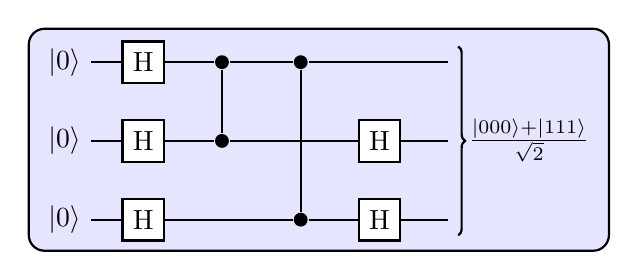
\begin{tikzpicture}[thick]
	%
	% `operator' will only be used by Hadamard (H) gates here.
	% `phase' is used for controlled phase gates (dots).
	% `surround' is used for the background box.
	\tikzstyle{operator} = [draw,fill=white,minimum size=1.5em] 
	\tikzstyle{phase} = [fill,shape=circle,minimum size=5pt,inner sep=0pt]
	\tikzstyle{surround} = [fill=blue!10,thick,draw=black,rounded corners=2mm]
	%
	% Qubits
	\node at (0,0) (q1) {\ket{0}};
	\node at (0,-1) (q2) {\ket{0}};
	\node at (0,-2) (q3) {\ket{0}};
	%
	% Column 1
	\node[operator] (op11) at (1,0) {H} edge [-] (q1);
	\node[operator] (op21) at (1,-1) {H} edge [-] (q2);
	\node[operator] (op31) at (1,-2) {H} edge [-] (q3);
	%
	% Column 3
	\node[phase] (phase11) at (2,0) {} edge [-] (op11);
	\node[phase] (phase12) at (2,-1) {} edge [-] (op21);
	\draw[-] (phase11) -- (phase12);
	%
	% Column 4
	\node[phase] (phase21) at (3,0) {} edge [-] (phase11);
	\node[phase] (phase23) at (3,-2) {} edge [-] (op31);
	\draw[-] (phase21) -- (phase23);
	%
	% Column 5
	\node[operator] (op24) at (4,-1) {H} edge [-] (phase12);
	\node[operator] (op34) at (4,-2) {H} edge [-] (phase23);
	%
	% Column 6
	\node (end1) at (5,0) {} edge [-] (phase21);
	\node (end2) at (5,-1) {} edge [-] (op24);
	\node (end3) at (5,-2) {} edge [-] (op34);
	%
	% Bracket
	\draw[decorate,decoration={brace},thick] (5,0.2) to
	node[midway,right] (bracket) {$\frac{\ket{000}+\ket{111}}{\sqrt{2}}$}
	(5,-2.2);
	%
	% Background Box
	\begin{pgfonlayer}{background} 
		\node[surround] (background) [fit = (q1) (op31) (bracket)] {};
	\end{pgfonlayer}
	%
\end{tikzpicture}
\end{document}
